\documentclass[a4paper]{article}
\usepackage{cmap}
\usepackage[utf8]{inputenc}
\usepackage[T2A]{fontenc}
\usepackage[english,russian]{babel} 
\usepackage[left=15mm, top=15mm, right=15mm, bottom=42mm, nohead, nofoot]{geometry}
\usepackage{blindtext}  % рыба-текст
\usepackage{graphicx}  % изобржаения
\usepackage{float} % плавающие объекты
\usepackage{wrapfig}  % изобржаения
\usepackage{tikz} % графика
\usepackage{xcolor} % определение цветов
\usepackage{nicefrac} % красивые дроби
\usepackage{cancel} % сокращение
\usepackage{amsmath,amsfonts,amssymb} % математический пакет
\usepackage{hyperref}  % гиперссылки
\usepackage{fancybox,fancyhdr} % хедер и футер
\usepackage{listings} % код
\usepackage{accsupp}
\usepackage{caption}
\captionsetup[figure]{name=Рисунок}
\pagestyle{fancy}
\fancyhf{}
\fancyhead[L]{Лабораторная работа №4}
\fancyhead[R]{\textit{Точностные свойства системы, астатизмы и регуляторы}}
\fancyfoot[C]{\thepage}
\headsep=8mm
\footskip=20mm

\definecolor{urlcolor}{HTML}{3454D1}
\definecolor{linkcolor}{HTML}{3454D1}
\hypersetup{pdfstartview=FitH, linkcolor=linkcolor, urlcolor=urlcolor, colorlinks=true}

\definecolor{strings}{rgb}{0,0.6,0}
\definecolor{comments}{rgb}{0,0.3,0}
\definecolor{numbers}{rgb}{0.5,0.5,0.5}
\definecolor{keywords}{rgb}{0.09,0.61,0.95}
\definecolor{background}{rgb}{0.97,0.97,0.97}
\newcommand{\noncopynumber}[1]{%
    \BeginAccSupp{method=escape,ActualText={}}%
    #1%
    \EndAccSupp{}%
}
\lstdefinestyle{codestyle}{
    backgroundcolor=\color{background},
    commentstyle=\color{comments},
    keywordstyle=\color{keywords},
    stringstyle=\color{strings},
    numberstyle=\tiny\color{numbers}\noncopynumber,
    basicstyle=\ttfamily\footnotesize,
    breakatwhitespace=false,
    breaklines=true,
    captionpos=b,
    inputencoding=utf8,
    keepspaces=true,
    numbers=left,
    numbersep=5pt,
    showspaces=false,
    showstringspaces=false,
    showtabs=false,
    tabsize=2,
    extendedchars=true,
    literate=
    {а}{{\cyra}}1
    {б}{{\cyrb}}1
    {в}{{\cyrv}}1
    {г}{{\cyrg}}1
    {д}{{\cyrd}}1
    {е}{{\cyre}}1
    {ж}{{\cyrzh}}1
    {з}{{\cyrz}}1
    {и}{{\cyri}}1
    {й}{{\cyrishrt}}1
    {к}{{\cyrk}}1
    {л}{{\cyrl}}1
    {м}{{\cyrm}}1
    {н}{{\cyrn}}1
    {о}{{\cyro}}1
    {п}{{\cyrp}}1
    {р}{{\cyrr}}1
    {с}{{\cyrs}}1
    {т}{{\cyrt}}1
    {у}{{\cyru}}1
    {ф}{{\cyrf}}1
    {х}{{\cyrh}}1
    {ц}{{\cyrc}}1
    {ч}{{\cyrch}}1
    {ш}{{\cyrsh}}1
    {щ}{{\cyrshch}}1
    {ъ}{{\cyrhrdsn}}1
    {ы}{{\cyrery}}1
    {ь}{{\cyrsftsn}}1
    {э}{{\cyrerev}}1
    {ю}{{\cyryu}}1
    {я}{{\cyrya}}1
    {А}{{\CYRA}}1
    {Б}{{\CYRB}}1
    {В}{{\CYRV}}1
    {Г}{{\CYRG}}1
    {Д}{{\CYR96}}1
    {Е}{{\CYRE}}1
    {Ж}{{\CYRZH}}1
    {З}{{\CYRZ}}1
    {И}{{\CYRI}}1
    {Й}{{\CYRISHRT}}1
    {К}{{\CYRK}}1
    {Л}{{\CYRL}}1
    {М}{{\CYRM}}1
    {Н}{{\CYRN}}1
    {О}{{\CYRO}}1
    {П}{{\CYRP}}1
    {Р}{{\CYRR}}1
    {С}{{\CYRS}}1
    {Т}{{\CYRT}}1
    {У}{{\CYRU}}1
    {Ф}{{\CYRF}}1
    {Х}{{\CYRH}}1
    {Ц}{{\CYRC}}1
    {Ч}{{\CYRCH}}1
    {Ш}{{\CYRSH}}1
    {Щ}{{\CYRSHCH}}1
    {Ъ}{{\CYRHRDSN}}1
    {Ы}{{\CYRERY}}1
    {Ь}{{\CYRSFTSN}}1
    {Э}{{\CYREREV}}1
    {Ю}{{\CYRYU}}1
    {Я}{{\CYRYA}}1
}

\lstset{style=codestyle}

\addto\captionsrussian{
  \renewcommand{\contentsname}
    {\centering Содержание}
}


\newlength{\tempheight}
\newcommand{\Let}{
\mathbin{\text{\settoheight{\tempheight}{\mathstrut}\raisebox{0.4\pgflinewidth}{
\tikz[baseline=0.5ex,line cap=round,line join=round] \draw (0,0) --++ (0.3em,0) --++ (0,2.3ex) --++ (-0.3em,0);
}}}}
\newcommand*\squared[1]{\tikz[baseline=(char.base)]{
            \node[shape=rectangle,draw,inner sep=4pt] (char) {#1};}}
\newcommand*\msquared[1]{\tikz[baseline=(char.base)]{
            \node[shape=rectangle,draw,inner sep=4pt] (char) {$\displaystyle #1$};}}
\newcommand{\at}{\biggr\rvert}
\newcommand{\shiftright}[3]{\makebox[#2][r]{\makebox[#1][l]{#3}}}
\newcommand{\e}{\;\text{e}}
\let\oldint\int
\def\int{\oldint\limits}
\DeclareRobustCommand{\divby}{%
  \mathrel{\vbox{\baselineskip.65ex\lineskiplimit0pt\hbox{.}\hbox{.}\hbox{.}}}%
}

\newcommand\NB{\textbf{N\kern-0.32em\textcolor{red}{B}}}

\begin{document}

\begin{titlepage}
    \begin{center}
        Федеральное государственное автономное образовательное \\ учреждение высшего образования \\[6pt]
        САНКТ-ПЕТЕРБУРГСКИЙ НАЦИОНАЛЬНЫЙ \\ ИССЛЕДОВАТЕЛЬСКИЙ УНИВЕРСИТЕТ ИТМО \\[16pt]
        Факультет систем управления и робототехники \\[26em]
        Лабораторная работа №4\\[0.5em]
        \textbf{ТОЧНОСТНЫЕ СВОЙСТВА СИСТЕМ, АСТАТИЗМЫ И РЕГУЛЯТОРЫ}
    \end{center}\,\\[10em]
    \begin{flushright}
        Студент: Заводин Е.Ю.\\
        Лин САУ R23 бак 1.1.1 \\[0.5em]
        Преподаватели: Перегудин А.А.\\
        Пашенко А.В.
    \end{flushright}\,\\[6em]
    \begin{center}
        {\small Санкт-Петербург \\ 2025}
    \end{center}
\end{titlepage}
\setcounter{page}{2}
\tableofcontents\newpage

\section{Задача стабилизации с идеальным дифференцирующим звеном}\

В задании рассматривается система 

$$\ddot{y}-\dot{y}+5y=u,$$
корни её характеристического полинома --- $\frac{1\pm\sqrt{19}i}{2}$.\ 

Зададим начальное условие $\dot{y}(0)=5$, промоделируем свободное движение разомкнутой системы ($u=0$):

\begin{figure}[H]
    \centering
    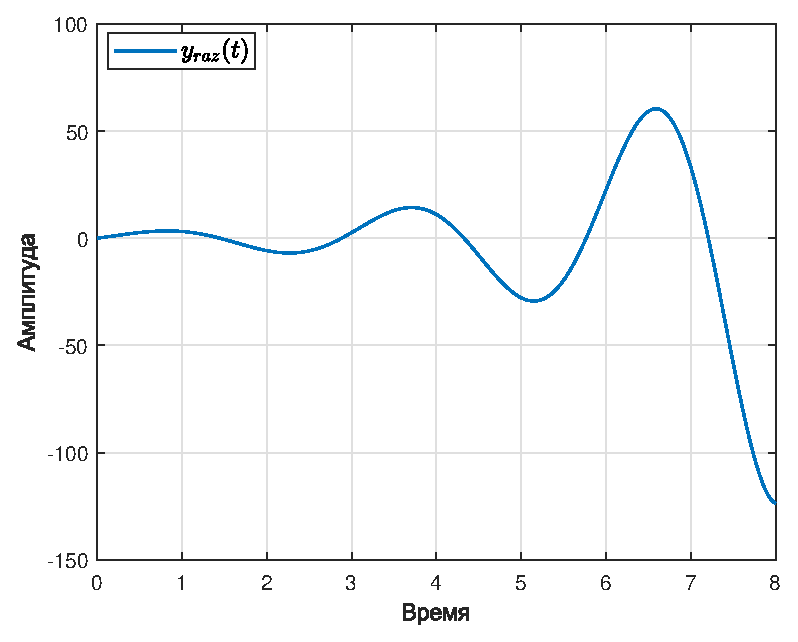
\includegraphics[width=0.6\linewidth]{ex1/razomk_fig.eps}
    \caption{Движение разомкнутой системы}
\end{figure}\

Заметно неустойчивое движение системы. Дабы устранить его, воспользуемся регулятором вида 

$$
u = k_0y + k_1\dot{y}.
$$\

Для моделирования движения системы с воздействием регулятора построим соответствующую структурную схему:

\begin{figure}[H]
    \centering
    \includegraphics[width=0.65\linewidth]{ex1/scheme_main.png}
    \caption{Структурная схема системы, замкнутой регулятором}
\end{figure}\

\begin{figure}[H]
    \centering
    \includegraphics[width=0.65\linewidth]{ex1/scheme_ws.png}
    \caption{Структурная схема объекта управления}
\end{figure}\

\begin{figure}[H]
    \centering
    \includegraphics[width=0.65\linewidth]{ex1/scheme_hs.png}
    \caption{Структурная схема регулятора}
\end{figure}\

Чтобы понять, какие значения $k_1, k_0$ выбрать для стабилизации движения системы, проанализируем передаточную функцию, получающуюся после воздействия регулятора.\ 

Передаточную функцию регулятора $W_{\text{рег}}(s)$ в действии на ПФ объекта управления $W_{\text{об}}(s)$ можно рассматривать как отдельную передаточную функцию замкнутой системы:

$$
W(s) = W_{\text{об}}(s)W_{\text{рег}}(s),
$$

$$
Y(s) = \frac{W(s)}{1+W(s)}.
$$\

Устойчивость линейной системы определяется расположением её полюсов: система устойчива, если все полюса лежат в левой полуплоскости комплексной плоскости. Полюса замкнутой системы --- корни знаменателя этой дроби, то есть решения уравнения

$$
1 + W(s) = 0 \Leftrightarrow 1 + W_{\text{об}}(s)W_{\text{рег}}(s) = 0.
$$

$$
\ddot{y} - \dot{y} + 5y = u \Leftrightarrow s^2y-sy+5y = u \Leftrightarrow y = \left(\frac{1}{s^2-s+5}\right)u \Rightarrow W_{\text{об}}(s) = \frac{1}{s^2-s+5}
$$

$$
u = k_0 y+k_1\dot{y} \Leftrightarrow u = k_0y + k_1sy \Leftrightarrow u = y(k_0 + k_1s) \Rightarrow W_{\text{рег}}(s) = k_0 + k_1s
$$

$$
1 + W_{\text{об}}(s)W_{\text{рег}}(s) = 1 + \frac{k_0 + k_1s}{s^2-s+5} = 1(s^2-s+5) + k_0+k_1s = s^2 + (k_1-1)s+(k_0+5)=0
$$\ 

Система будет асимптотически устойчива, если $k_0+5 > 0 \Leftrightarrow k_0 > -5$ и $k_1-1 > 0 \Leftrightarrow k_1 > 1$. При $k_0 = -5, k_1 = 1$ система устойчива по Ляпунову.\ 

Примем $k_0 = 1, k_1 = 3$, промоделируем систему при таких значениях параметров:

\begin{figure}[H]
    \centering
    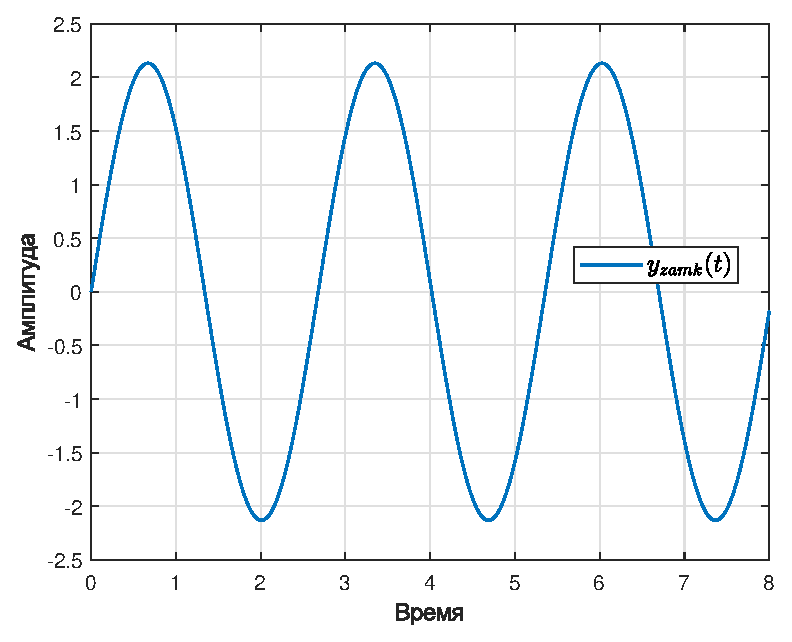
\includegraphics[width=0.65\linewidth]{ex1/zamk_fig.eps}
    \caption{Движение системы, замкнутой регулятором}
\end{figure}\

Видим, что теперь система асимптотически устойчива с установившимся значением $y_{\text{уст}} = 0$, таким образом получилось стабилизировать неустойчивую систему.

\section{Задача стабилизации с реальным дифференцирующим звеном}\

В задании аппроксимация производной при помощи блока $\text{Derivative}$ заменяется передаточной функцией

$$
W_{\text{р.дифф.}}(p) = \frac{p}{Tp+1}.
$$\

Это значит, что меняется и передаточная функция $W_{\text{рег}}(s)$, с учётом введения в него новой передаточной функции он начинает выглядеть следующим образом:

$$
W_{\text{рег}} = k_0+k_1\frac{s}{Ts+1}.
$$\ 

Проанализируем, при каких $T$ система будет неустойчива, по аналогии с предыдущим заданием воспользовавшись анализом корней знаменателя передаточной функции замкнутой системы:

$$
W(s) = \left(k_0 + k_1 \frac{s}{T s + 1}\right) \cdot \frac{1}{s^2 - s + 5} = \frac{(k_0 T + k_1)s + k_0}{T s + 1}\cdot \frac{1}{s^2 - s + 5} = \frac{(k_0 T + k_1)s + k_0}{(T s + 1)(s^2 - s + 5)}.
$$\

Тогда
$$
1 + W(s) = 0 \quad \Rightarrow \quad (T s + 1)(s^2 - s + 5) + (k_0 T + k_1)s + k_0 = 0.
$$\ 

Раскроем скобки:  
$$
(T s + 1)(s^2 - s + 5) = T s(s^2 - s + 5) + 1\cdot(s^2 - s + 5)=
$$
$$
= T s^3 - T s^2 + 5T s + s^2 - s + 5=
$$
$$
= T s^3 + (1 - T)s^2 + (5T - 1)s + 5.
$$\

$$
T s^3 + (1-T)s^2 + (5T - 1 + k_0 T + k_1)s + (5 + k_0) = 0.
$$\ 

Подставим выбранные $k_0 = 1, k_1 = 3$:

$$
T s^3 + (1-T)s^2 + (5T + T + 2)s + 6 = 0 \Leftrightarrow s^3 + \frac{1-T}{T}s^2 + \left(\frac{2}{T} + 6\right)s + \frac{6}{T} = 0
$$\

По критерию Гурвица кубический полином устойчив, если $a_2, a_1, a_0 > 0$ и $a_2 a_1 > a_0$. В нашем случае система асимптотически устойчива, если выполнены следующие условия:

$$
a_0 = \frac{6}{T} > 0 \Leftrightarrow T > 0
$$
$$
a_1 = \frac{2}{T} + 6 > 0 \Leftrightarrow T > -\frac{2}{6}, T\neq0
$$
$$
a_2 = \frac{1 - T}{T} > 0 \Leftrightarrow 1 - T > 0, \Leftrightarrow T < 1
$$\ 

$$a_2 a_1 > a_0 \Leftrightarrow
\left(\frac{1 - T}{T}\right) \left(\frac{2}{T} + 6\right) > \frac{6}{T}.
$$\ 

Из условий выше знаем, что $T > 0$, значит, можем домножить на $T$:

\[
(1 - T)\left(\frac{2}{T} + 6\right) > 6.
\]

Раскрывая скобки, получим:

\[
(1 - T)\cdot\frac{2}{T} + (1 - T)\cdot6 > 6\Leftrightarrow
\frac{2(1 - T)}{T} + 6(1 - T) > 6\Leftrightarrow
\]

\[
\frac{2(1 - T)}{T} + 6(1 - T) - 6 > 0\Leftrightarrow
\frac{2(1 - T)}{T} + 6(1 - T - 1) > 0\Leftrightarrow
\frac{2(1 - T)}{T} - 6T > 0.
\]

Приведём к общему знаменателю \(T > 0\):

\[
\frac{2(1 - T) - 6T^2}{T} > 0.
\]

Числитель:

\[
2(1 - T) - 6T^2 = 2 - 2T - 6T^2.
\]

Неравенство:

\[
\frac{-6T^2 - 2T + 2}{T} > 0.
\]

Рассмотрим числитель:  
\[
-6T^2 - 2T + 2 = -2(3T^2 + T - 1).
\]

Корни уравнения \(3T^2 + T - 1 = 0\):

\[
T_{1, 2} = \frac{-1 \pm \sqrt{13}}{6}.
\]\ 

Ветви соответствующей уравнению параболы направлены вверх, а значит, система неустойчива при $T \ge \frac{-1 + \sqrt{13}}{6}$ и при $T\le \frac{-1 - \sqrt{13}}{6}$.\ Итого, сопоставляя полученные ограничения на $T$, получаем отрезок, в котором система асимптотически устойчива: $T \in \left(0, \frac{-1 + \sqrt{13}}{6}\right)$

Система была промоделирована для нескольких различных значений параметра $T$, соответствующих устойчивой системе:

\begin{figure}[H]
    \centering
    \includegraphics[width=0.65\linewidth]{ex2/all.eps}
    \caption{Движение системы при разных $T$, в сравнении с результатом моделирования из задания 1}
\end{figure}\

Заметно, что чем ближе $T$ к 0, тем ближе соответствующая траектория к траектории $y_{zamk}(t)$, полученной в первом задании. Также чем ближе $T$ к своей верхней границе, тем сильнее расходится траектория движения системы. Отдельно промоделирую систему на верхней границе, $T = \frac{-1 + \sqrt{13}}{6}\approx 0.434$:

\begin{figure}[H]
    \centering
    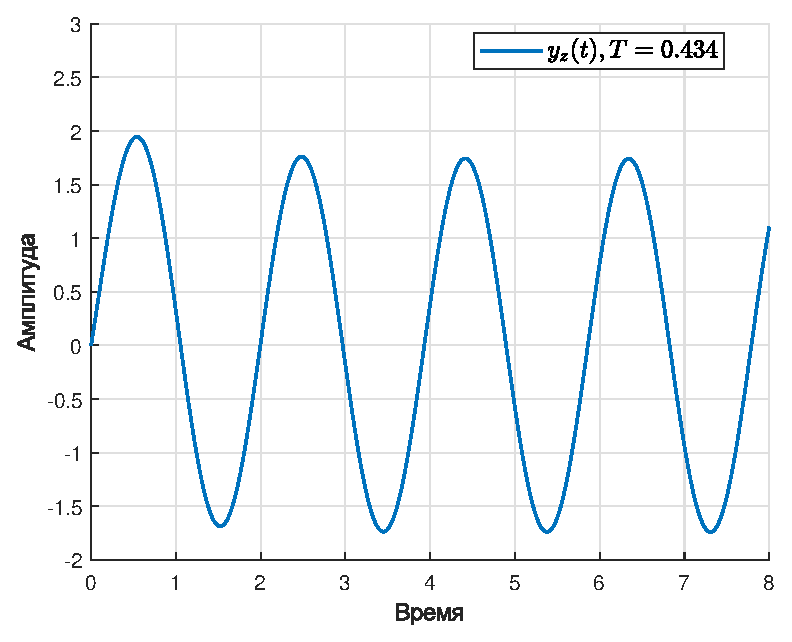
\includegraphics[width=0.65\linewidth]{ex2/0.434.eps}
    \caption{Движение системы при граничном значении $T$}
\end{figure}\

Видно, что траектория движения системы больше походит на устойчивую по Ляпунову, чем на асимптотическую.

\subsection{Вывод}

Я понял, что добавление в регулятор дифференцирующего звена меняет его передаточную функцию, и понял, как определить устойчивость системы исходя из параметра добавленного звена. 

\section{Задача слежения для системы с астатизмом нулевого порядка (П-регулятор)}\

Рассмотрим замкнутую систему, заданную структурной схемой, отображённой на рисунке:

\begin{figure}[H]
    \centering
    \includegraphics[width=0.65\linewidth]{ex3/image.png}
    \caption{Структурная схема с П-регулятором}
\end{figure}\

Передаточная функция системы --- $W_s(s) = \frac{5}{s^2+5s+6}$, регулятором выступает $H(s) = k$. Для значения параметра регулятора был выбран набор значений $[1, 3, 7]$.\ 

\subsection{Стационарная желаемая функция}

Исследование стационарного режима работы проводится с задающим воздействием $g(t) = 1$. Для этого режима при выбранной передаточной функции объекта управления и регулятора можно будет найти установившееся значение ошибки (система обладает нулевым порядком астатизма, а значит, при $t \to \infty$ между траекторией движения системы и задающим воздействием будет фиксированная величина $e_\text{уст}$).\ 

Для расчёта установившейся ошибки понадобится вычислить передаточную функцию разомкнутой системы:

$$
W(s) = W_s(s) H(s) = \frac{5k}{s^2+5s+6}
$$\ 

Зная передаточную функцию разомкнутой системы, можем построить передаточную функцию по ошибке слежения:

$$
\underset{g\to e}{W}(s) = \frac{1}{1+W(s)} = \frac{1}{1+\frac{5k}{s^2+5s+6}}=\frac{s^2+5s+6}{s^2+5s+6+5k}
$$\ 

Тогда образ Лапласа ошибки слежения будет определяться как 

$$
E(s) = \underset{g\to e}{W}(s) \cdot G(s),
$$
где $G(s) = \frac{1}{s}$ -- образ Лапласа от задающего воздействия $g(t) = 1$.

$$
E(s) = \frac{s^2+5s+6}{s(s^2+5s+6+5k)}.
$$\ 

Пользуясь теоремой о конечном значении, можем вычислить непосредственно установившуюся ошибку:

$$
e_{\text{уст}} = \lim_{t\to \infty} e(t) = \lim_{s\to 0} sE(s) = \lim_{s\to 0}\frac{\cancel{s}\left(s^2+5s+6\right)}{\cancel{s}\left(s^2+5s+6+5k\right)} = \frac{\cancelto{0}{s^2}+5\cancelto{0}{s}+6}{\cancelto{0}{s^2}+5\cancelto{0}{s}+6+5k} =\frac{6}{6+5k}
$$\ 

Тогда для $k = 1$ $e_{\text{уст}} = \frac{6}{11}$, для $k = 3$: $e_{\text{уст}} = \frac{6}{21}$, для $k = 7$: $e_{\text{уст}} = \frac{6}{41}$.\ 

То есть чем больше $k$, тем ближе он к 0.\ 

Проверим теорию на ``практике'':

\begin{figure}[H]
    \begin{minipage}{0.5\textwidth}
        \centering 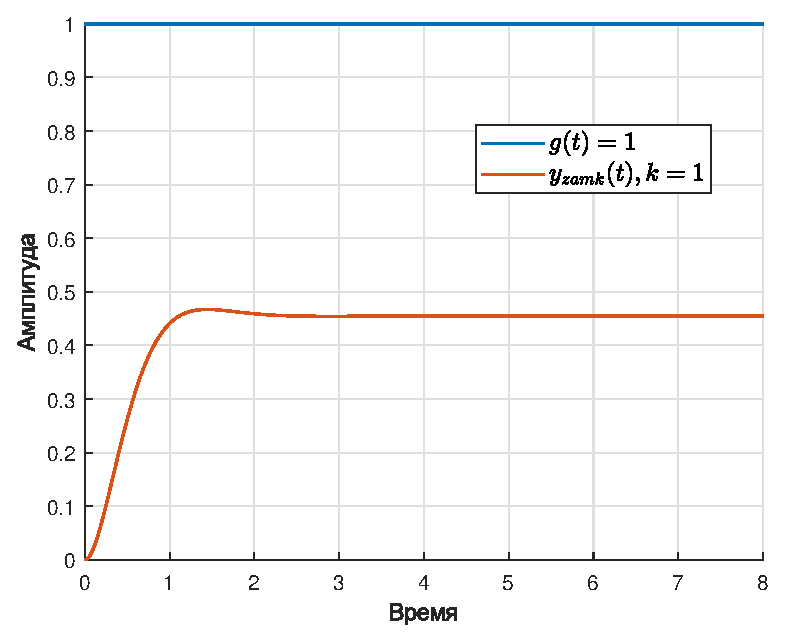
\includegraphics[width=\textwidth]{ex3/k1_g_a.eps}
        \caption{Сопоставление графиков выхода и входа для}
        \centerline{$k=1$, $g=1$}
    \end{minipage}\hfill
    \begin{minipage}{0.5\textwidth}
        \centering 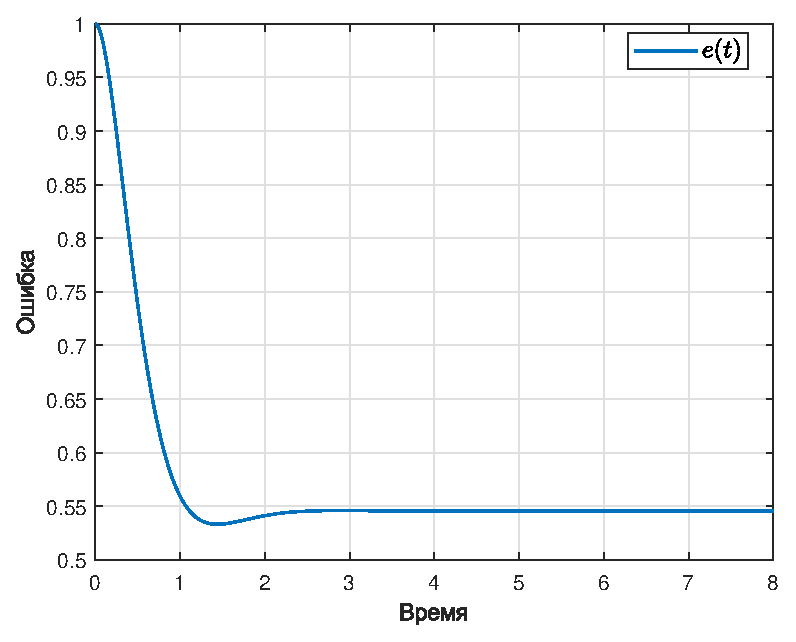
\includegraphics[width=\textwidth]{ex3/k1_g_a_error.eps}
        \caption{График ошибки для $k=1$, $g=1$}
        % \centerline{лягушки}
    \end{minipage}\\[1em]
\end{figure}\noindent\

В этом случае установившаяся ошибка совпадает с предсказанной $e_{\text{уст}} =\frac{6}{11} \approx 0.55$.

\begin{figure}[H]
    \begin{minipage}{0.5\textwidth}
        \centering 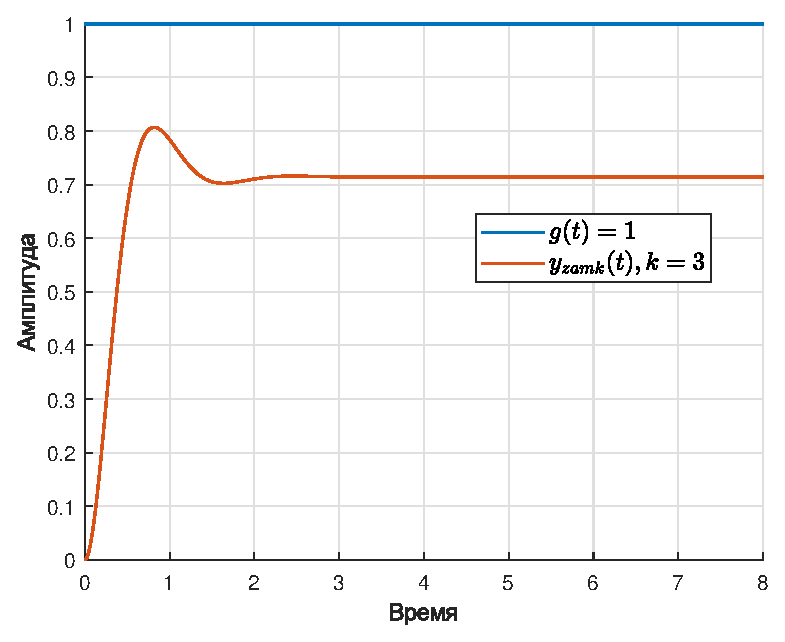
\includegraphics[width=\textwidth]{ex3/k3_g_a.eps}
        \caption{Сопоставление графиков выхода и входа для}
        \centerline{$k=3$, $g=1$}
    \end{minipage}\hfill
    \begin{minipage}{0.5\textwidth}
        \centering 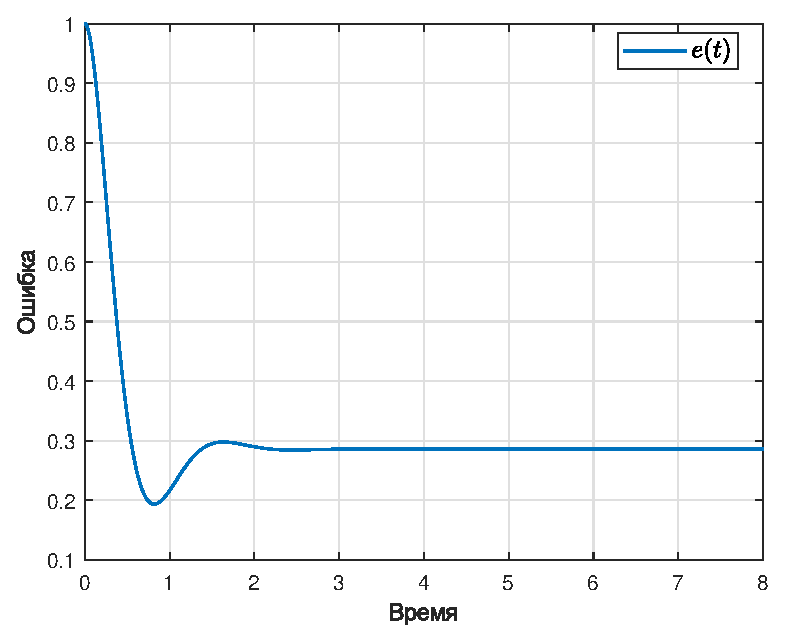
\includegraphics[width=\textwidth]{ex3/k3_g_a_error.eps}
        \caption{График ошибки для $k=3$, $g=1$}
        % \centerline{лягушки}
    \end{minipage}\\[1em]
\end{figure}\noindent\

В этом случае установившаяся ошибка также совпадает с предсказанной $e_{\text{уст}} =\frac{6}{21} \approx 0.29$.

\begin{figure}[H]
    \begin{minipage}{0.5\textwidth}
        \centering 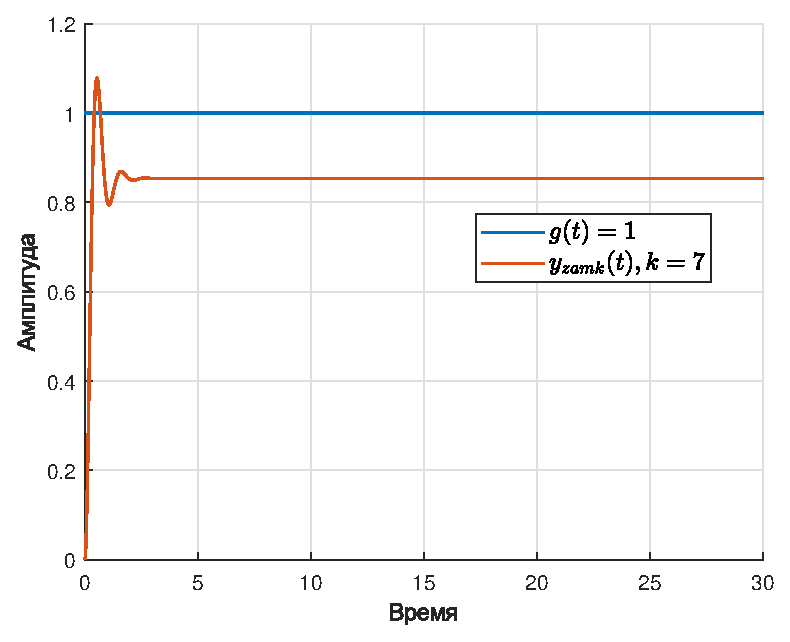
\includegraphics[width=\textwidth]{ex3/k7_g_a.eps}
        \caption{Сопоставление графиков выхода и входа для}
        \centerline{$k=7$, $g=1$}
    \end{minipage}\hfill
    \begin{minipage}{0.5\textwidth}
        \centering 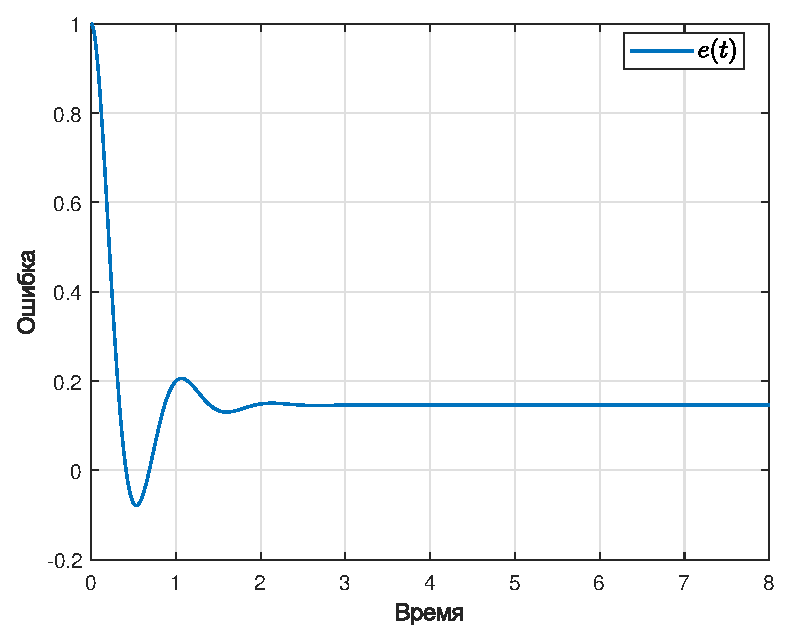
\includegraphics[width=\textwidth]{ex3/k7_g_a_error.eps}
        \caption{График ошибки для $k=7$, $g=1$}
        % \centerline{лягушки}
    \end{minipage}\\[1em]
\end{figure}\noindent\

В этом случае установившаяся ошибка снова совпадала с предсказанной $e_{\text{уст}} =\frac{6}{41} \approx 0.16$.

Во всех трёх случаях ошибка сошлась к константе, как и ожидалось. Заметно, что чем больше $k$, тем меньше установившаяся ошибка, но в то же время и больше перерегулирование, и тем больше колебательности появляется у конечного сигнала.

\subsection{Функция с постоянной скоростью}\

В этой части задания на вход подаётся линейно растущее воздействие -- $g(t) = t$. В этом случае из-за низкого порядка астатизма система не сможет ни свести ошибку слежения к 0, ни прийти к установившемуся значению этой ошибки: 

\begin{figure}[H]
    \begin{minipage}{0.5\textwidth}
        \centering 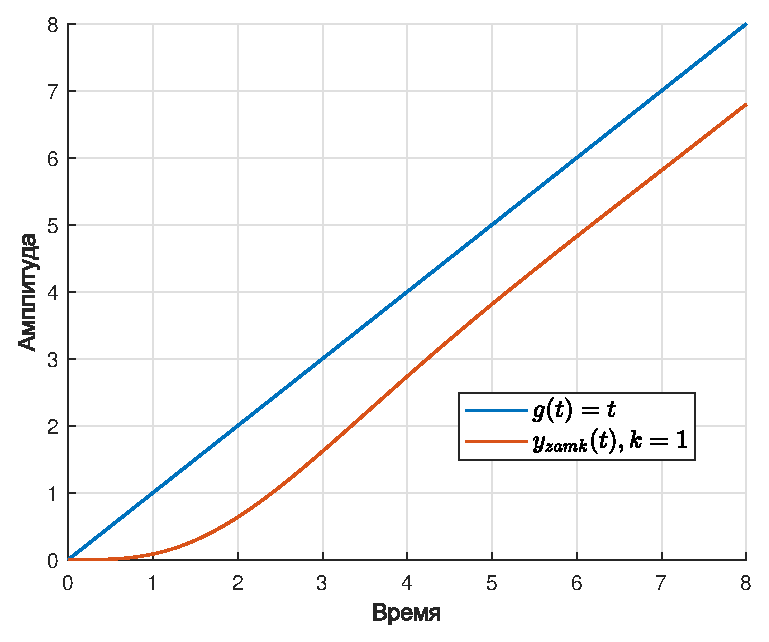
\includegraphics[width=\textwidth]{ex3/k1_g_vt.eps}
        \caption{Сопоставление графиков выхода и входа для}
        \centerline{$k=1$, $g=t$}
    \end{minipage}\hfill
    \begin{minipage}{0.5\textwidth}
        \centering 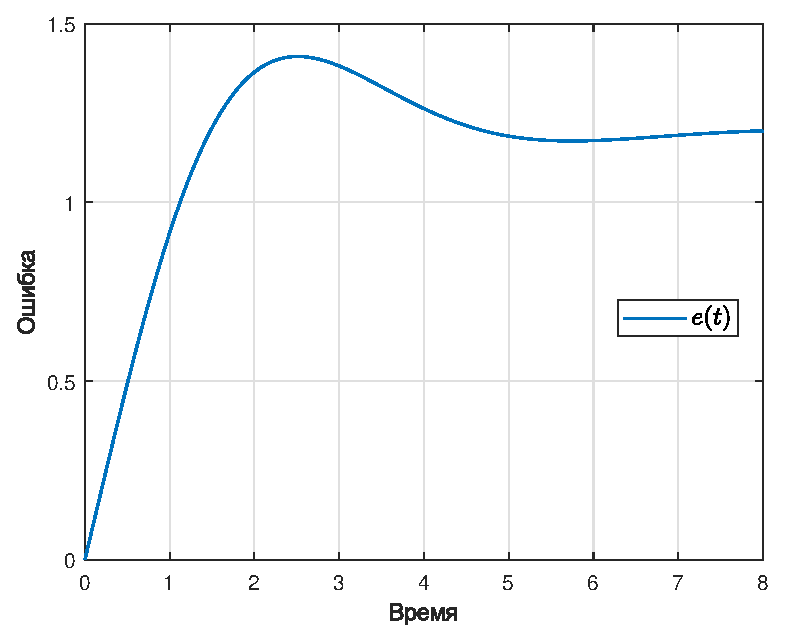
\includegraphics[width=\textwidth]{ex3/k1_g_vt_error.eps}
        \caption{График ошибки для $k=1$, $g=t$}
        % \centerline{лягушки}
    \end{minipage}\\[1em]
\end{figure}\noindent\

\begin{figure}[H]
    \begin{minipage}{0.5\textwidth}
        \centering 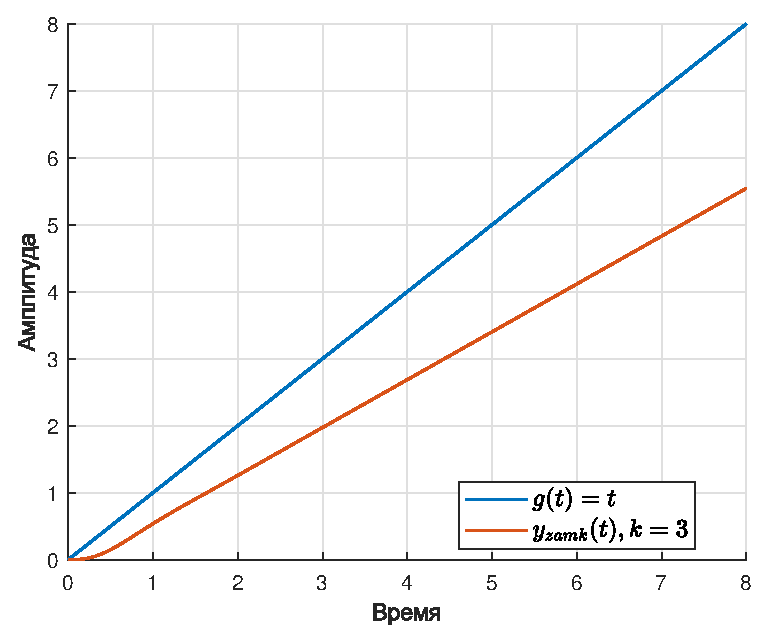
\includegraphics[width=\textwidth]{ex3/k3_g_vt.eps}
        \caption{Сопоставление графиков выхода и входа для}
        \centerline{$k=3$, $g=t$}
    \end{minipage}\hfill
    \begin{minipage}{0.5\textwidth}
        \centering 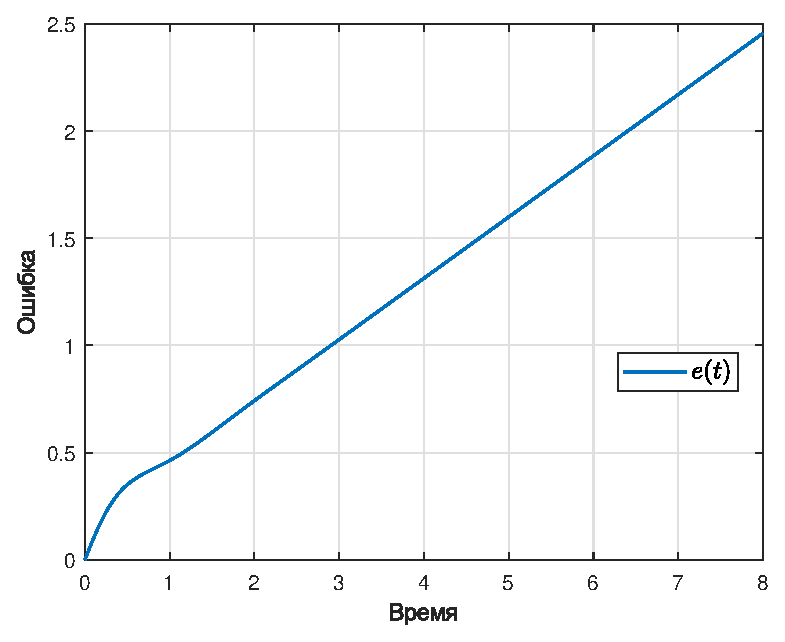
\includegraphics[width=\textwidth]{ex3/k3_g_vt_error.eps}
        \caption{График ошибки для $k=3$, $g=t$}
        % \centerline{лягушки}
    \end{minipage}\\[1em]
\end{figure}\noindent\

\begin{figure}[H]
    \begin{minipage}{0.5\textwidth}
        \centering 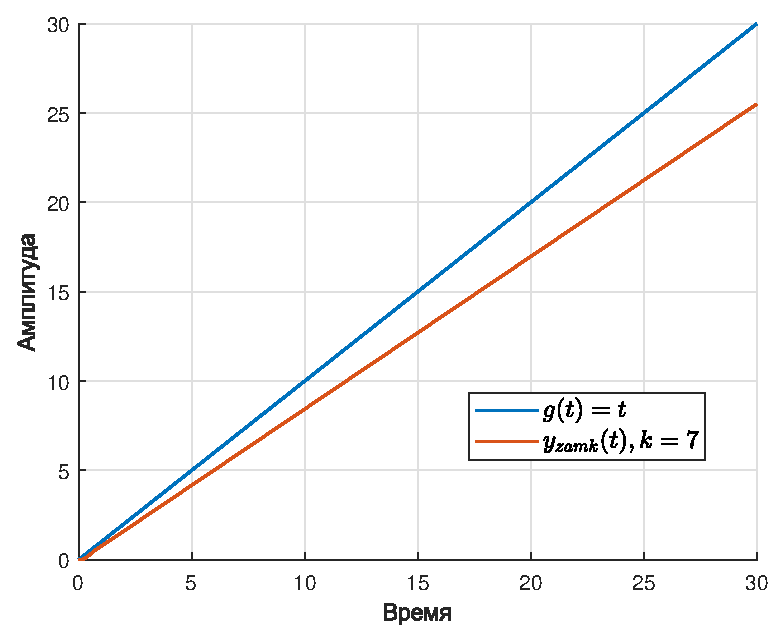
\includegraphics[width=\textwidth]{ex3/k7_g_vt.eps}
        \caption{Сопоставление графиков выхода и входа для}
        \centerline{$k=7$, $g=t$}
    \end{minipage}\hfill
    \begin{minipage}{0.5\textwidth}
        \centering 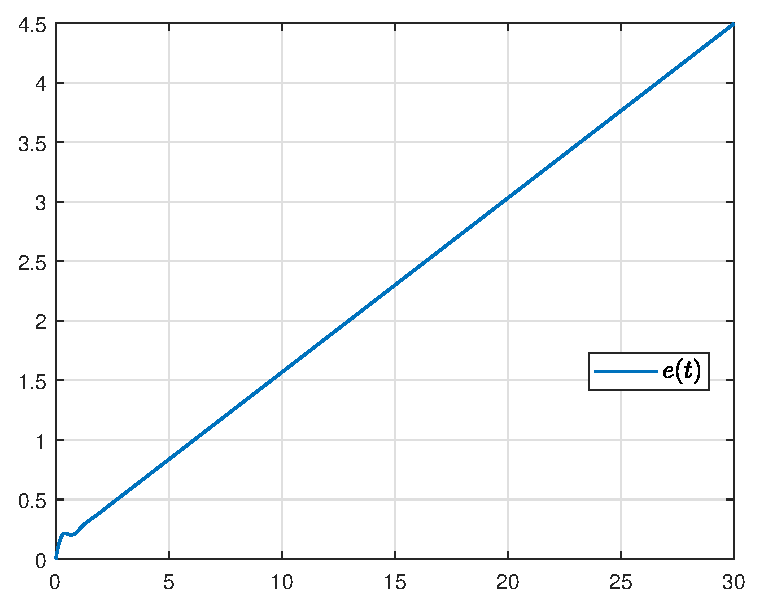
\includegraphics[width=\textwidth]{ex3/k7_g_vt_error.eps}
        \caption{График ошибки для $k=7$, $g=t$}
        % \centerline{лягушки}
    \end{minipage}\\[1em]
\end{figure}\noindent\


\section{Задача слежения для системы с астатизмом первого порядка (И-регулятор)}\

\section{Задача слежения для системы с астатизмом первого порядка (ПИ-регулятор)}\

\section{Задача слежения за гармоническим сигналом (регулятор общего вида)}\

\section{Приложение А. Код для выполнения заданий}

\subsection*{Листинг 1. Код для выполнения задания 1}

\begin{lstlisting}[caption={Код для построения графиков для задания 1}, language=matlab]
% clear all;
close all;

[~, scriptName] = fileparts(mfilename('fullpath'));
if ~isfolder(scriptName)
    mkdir(scriptName);
end

t = (0:0.01:8)';
% u = [t, 1.5*ones(size(t))];
% u = [t, 0.6*t];
u = [t, zeros(size(t))];

fig_svob = figure;
out = sim('ex1/model.slx','StopTime','8');
y_model = out.y;
plot(y_model.Time, y_model.Data, LineWidth=1.2, DisplayName="$y_{raz}(t)$")
xlabel('Время'), ylabel('Амплитуда')
grid on
legend(Interpreter='latex', Location='best', BackgroundAlpha=.1, FontSize=12, FontName='Computer Modern')
saveas(fig_svob, string(scriptName) + '\' + 'razomk_fig' + '.eps', 'epsc')

k0 = 1;
k1 = 3; % траектория становится ограниченной при k1 = 1, k1 > 1 - система Ау, k1 < 1 - Ну

fig_regulator = figure;
out = sim('ex1/model_regulator.slx','StopTime','8');
y_model = out.y;
plot(y_model.Time, y_model.Data, LineWidth=1.2, DisplayName="$y_{zamk}(t)$")
xlabel('Время'), ylabel('Амплитуда')
grid on
legend(Interpreter='latex', Location='best', BackgroundAlpha=.1, FontSize=12, FontName='Computer Modern')
saveas(fig_regulator, string(scriptName) + '\' + 'zamk_fig' + '.eps', 'epsc')


% figure;
% num = [1];
% den = [1 -4 5];
% sys = tf(num, den);
% y = lsim(sys, u(:,2), t);
% plot(t, y)
\end{lstlisting}
\subsection*{Листинг 1. Код для выполнения задания 1}

\begin{lstlisting}[caption={Код для построения графиков для задания 2}, language=matlab]
% clear all;
close all;

[~, scriptName] = fileparts(mfilename('fullpath'));
if ~isfolder(scriptName)
    mkdir(scriptName);
end

t = (0:0.01:8)';
% u = [t, 1.5*ones(size(t))];
% u = [t, 0.6*t];
u = [t, zeros(size(t))];

T = 0.01;

k0 = 1;
k1 = 3; % траектория становится ограниченной при k1 = 1, k1 > 1 - система Ау, k1 < 1 - Ну

fig_regulator = figure;
hold on; grid on;

out = sim('ex1/model_regulator.slx','StopTime','8');
y_model = out.y;
plot(y_model.Time, y_model.Data, LineWidth=1.5, DisplayName="$y_{zamk}(t)$", Color='black')

out = sim('ex2/model_regulator2.slx','StopTime','8');
y_model = out.y;
plot(y_model.Time, y_model.Data, LineWidth=1.3, DisplayName="$y_{z}(t), T = " + string(T) + "$")
T = 0.4;

out = sim('ex2/model_regulator2.slx','StopTime','8');
y_model = out.y;
plot(y_model.Time, y_model.Data, LineWidth=1.3, DisplayName="$y_{z}(t), T = " + string(T) + "$")

T = 0.2;
out = sim('ex2/model_regulator2.slx','StopTime','8');
y_model = out.y;
plot(y_model.Time, y_model.Data, LineWidth=1.3, DisplayName="$y_{z}(t), T = " + string(T) + "$")

T = 0.1;
out = sim('ex2/model_regulator2.slx','StopTime','8');
y_model = out.y;
plot(y_model.Time, y_model.Data, LineWidth=1.3, DisplayName="$y_{z}(t), T = " + string(T) + "$")

xlabel('Время'), ylabel('Амплитуда')
ylim([-2, 3])
legend(Interpreter='latex', Location='best', BackgroundAlpha=.3, FontSize=12, FontName='Computer Modern')
saveas(fig_regulator, string(scriptName) + '\' + string(T) + '.eps', 'epsc')
\end{lstlisting}


\end{document}
